% Options for packages loaded elsewhere
\PassOptionsToPackage{unicode}{hyperref}
\PassOptionsToPackage{hyphens}{url}
%
\documentclass[
]{article}
\usepackage{lmodern}
\usepackage{amssymb,amsmath}
\usepackage{ifxetex,ifluatex}
\ifnum 0\ifxetex 1\fi\ifluatex 1\fi=0 % if pdftex
  \usepackage[T1]{fontenc}
  \usepackage[utf8]{inputenc}
  \usepackage{textcomp} % provide euro and other symbols
\else % if luatex or xetex
  \usepackage{unicode-math}
  \defaultfontfeatures{Scale=MatchLowercase}
  \defaultfontfeatures[\rmfamily]{Ligatures=TeX,Scale=1}
\fi
% Use upquote if available, for straight quotes in verbatim environments
\IfFileExists{upquote.sty}{\usepackage{upquote}}{}
\IfFileExists{microtype.sty}{% use microtype if available
  \usepackage[]{microtype}
  \UseMicrotypeSet[protrusion]{basicmath} % disable protrusion for tt fonts
}{}
\makeatletter
\@ifundefined{KOMAClassName}{% if non-KOMA class
  \IfFileExists{parskip.sty}{%
    \usepackage{parskip}
  }{% else
    \setlength{\parindent}{0pt}
    \setlength{\parskip}{6pt plus 2pt minus 1pt}}
}{% if KOMA class
  \KOMAoptions{parskip=half}}
\makeatother
\usepackage{xcolor}
\IfFileExists{xurl.sty}{\usepackage{xurl}}{} % add URL line breaks if available
\IfFileExists{bookmark.sty}{\usepackage{bookmark}}{\usepackage{hyperref}}
\hypersetup{
  pdftitle={Wrkshp2\_RMarkdown},
  pdfauthor={Katherine Castrillon},
  hidelinks,
  pdfcreator={LaTeX via pandoc}}
\urlstyle{same} % disable monospaced font for URLs
\usepackage[margin=1in]{geometry}
\usepackage{graphicx,grffile}
\makeatletter
\def\maxwidth{\ifdim\Gin@nat@width>\linewidth\linewidth\else\Gin@nat@width\fi}
\def\maxheight{\ifdim\Gin@nat@height>\textheight\textheight\else\Gin@nat@height\fi}
\makeatother
% Scale images if necessary, so that they will not overflow the page
% margins by default, and it is still possible to overwrite the defaults
% using explicit options in \includegraphics[width, height, ...]{}
\setkeys{Gin}{width=\maxwidth,height=\maxheight,keepaspectratio}
% Set default figure placement to htbp
\makeatletter
\def\fps@figure{htbp}
\makeatother
\setlength{\emergencystretch}{3em} % prevent overfull lines
\providecommand{\tightlist}{%
  \setlength{\itemsep}{0pt}\setlength{\parskip}{0pt}}
\setcounter{secnumdepth}{-\maxdimen} % remove section numbering

\title{Wrkshp2\_RMarkdown}
\author{Katherine Castrillon}
\date{1/24/2020}

\begin{document}
\maketitle

\hypertarget{objectives}{%
\section{Objectives}\label{objectives}}

The site of observation is a mixed temperate forest, the Harvard Forest.
The data utilized in this analyses was taken from the Harvard dataframe
using flux data from Ameriflux for the Harvard Forest tower (Ha1). The
harv dataset was divided into: day (PAR\textgreater0) and night
(PAR==0). In this analysis, the night (PAR==0) dataframe was utilized
for understanding annual patterns ecosystem photosynthetic potential and
respiration rates in temperate mixed forest; observed data was collected
for every year from 1991 to 2016.

Net Ecosystem Exchange (NEE) rates of temperature were quantified for
the night dataframe (nee.night) to determine the varibale rates of NEE
on an annual basis.

The purpose of looking at flux data from Ameriflux for the Harvard
Forest tower (Ha1) was to understand annual patterns of the ecosystems
photosynthetic potential and occurring respiration rates within the
temperate mixed forest. Net Ecosystem Exchange (NEE) rates was used to
quantify for the given night dataframe (nee.night) to determine the
variable rates of NEE on an annual basis.

Methodology used to determine respiration in regards to temperature
required for use of the creation of a dataframe to store monthly
parameters (parms.Month), writing a funtion to fit the model and extract
parameter values from nee.night, writing a loop to fit monthly curves
and add parameters to the parms.Month dataframe, and error estimation by
use of bootstrapping.

\#Methods

The observed site was Harvard Forest, NEE data taken from Harvard Forest
tower Ha1, located at Lat/Long 42.5369, -72.17266.

\begin{figure}
\centering
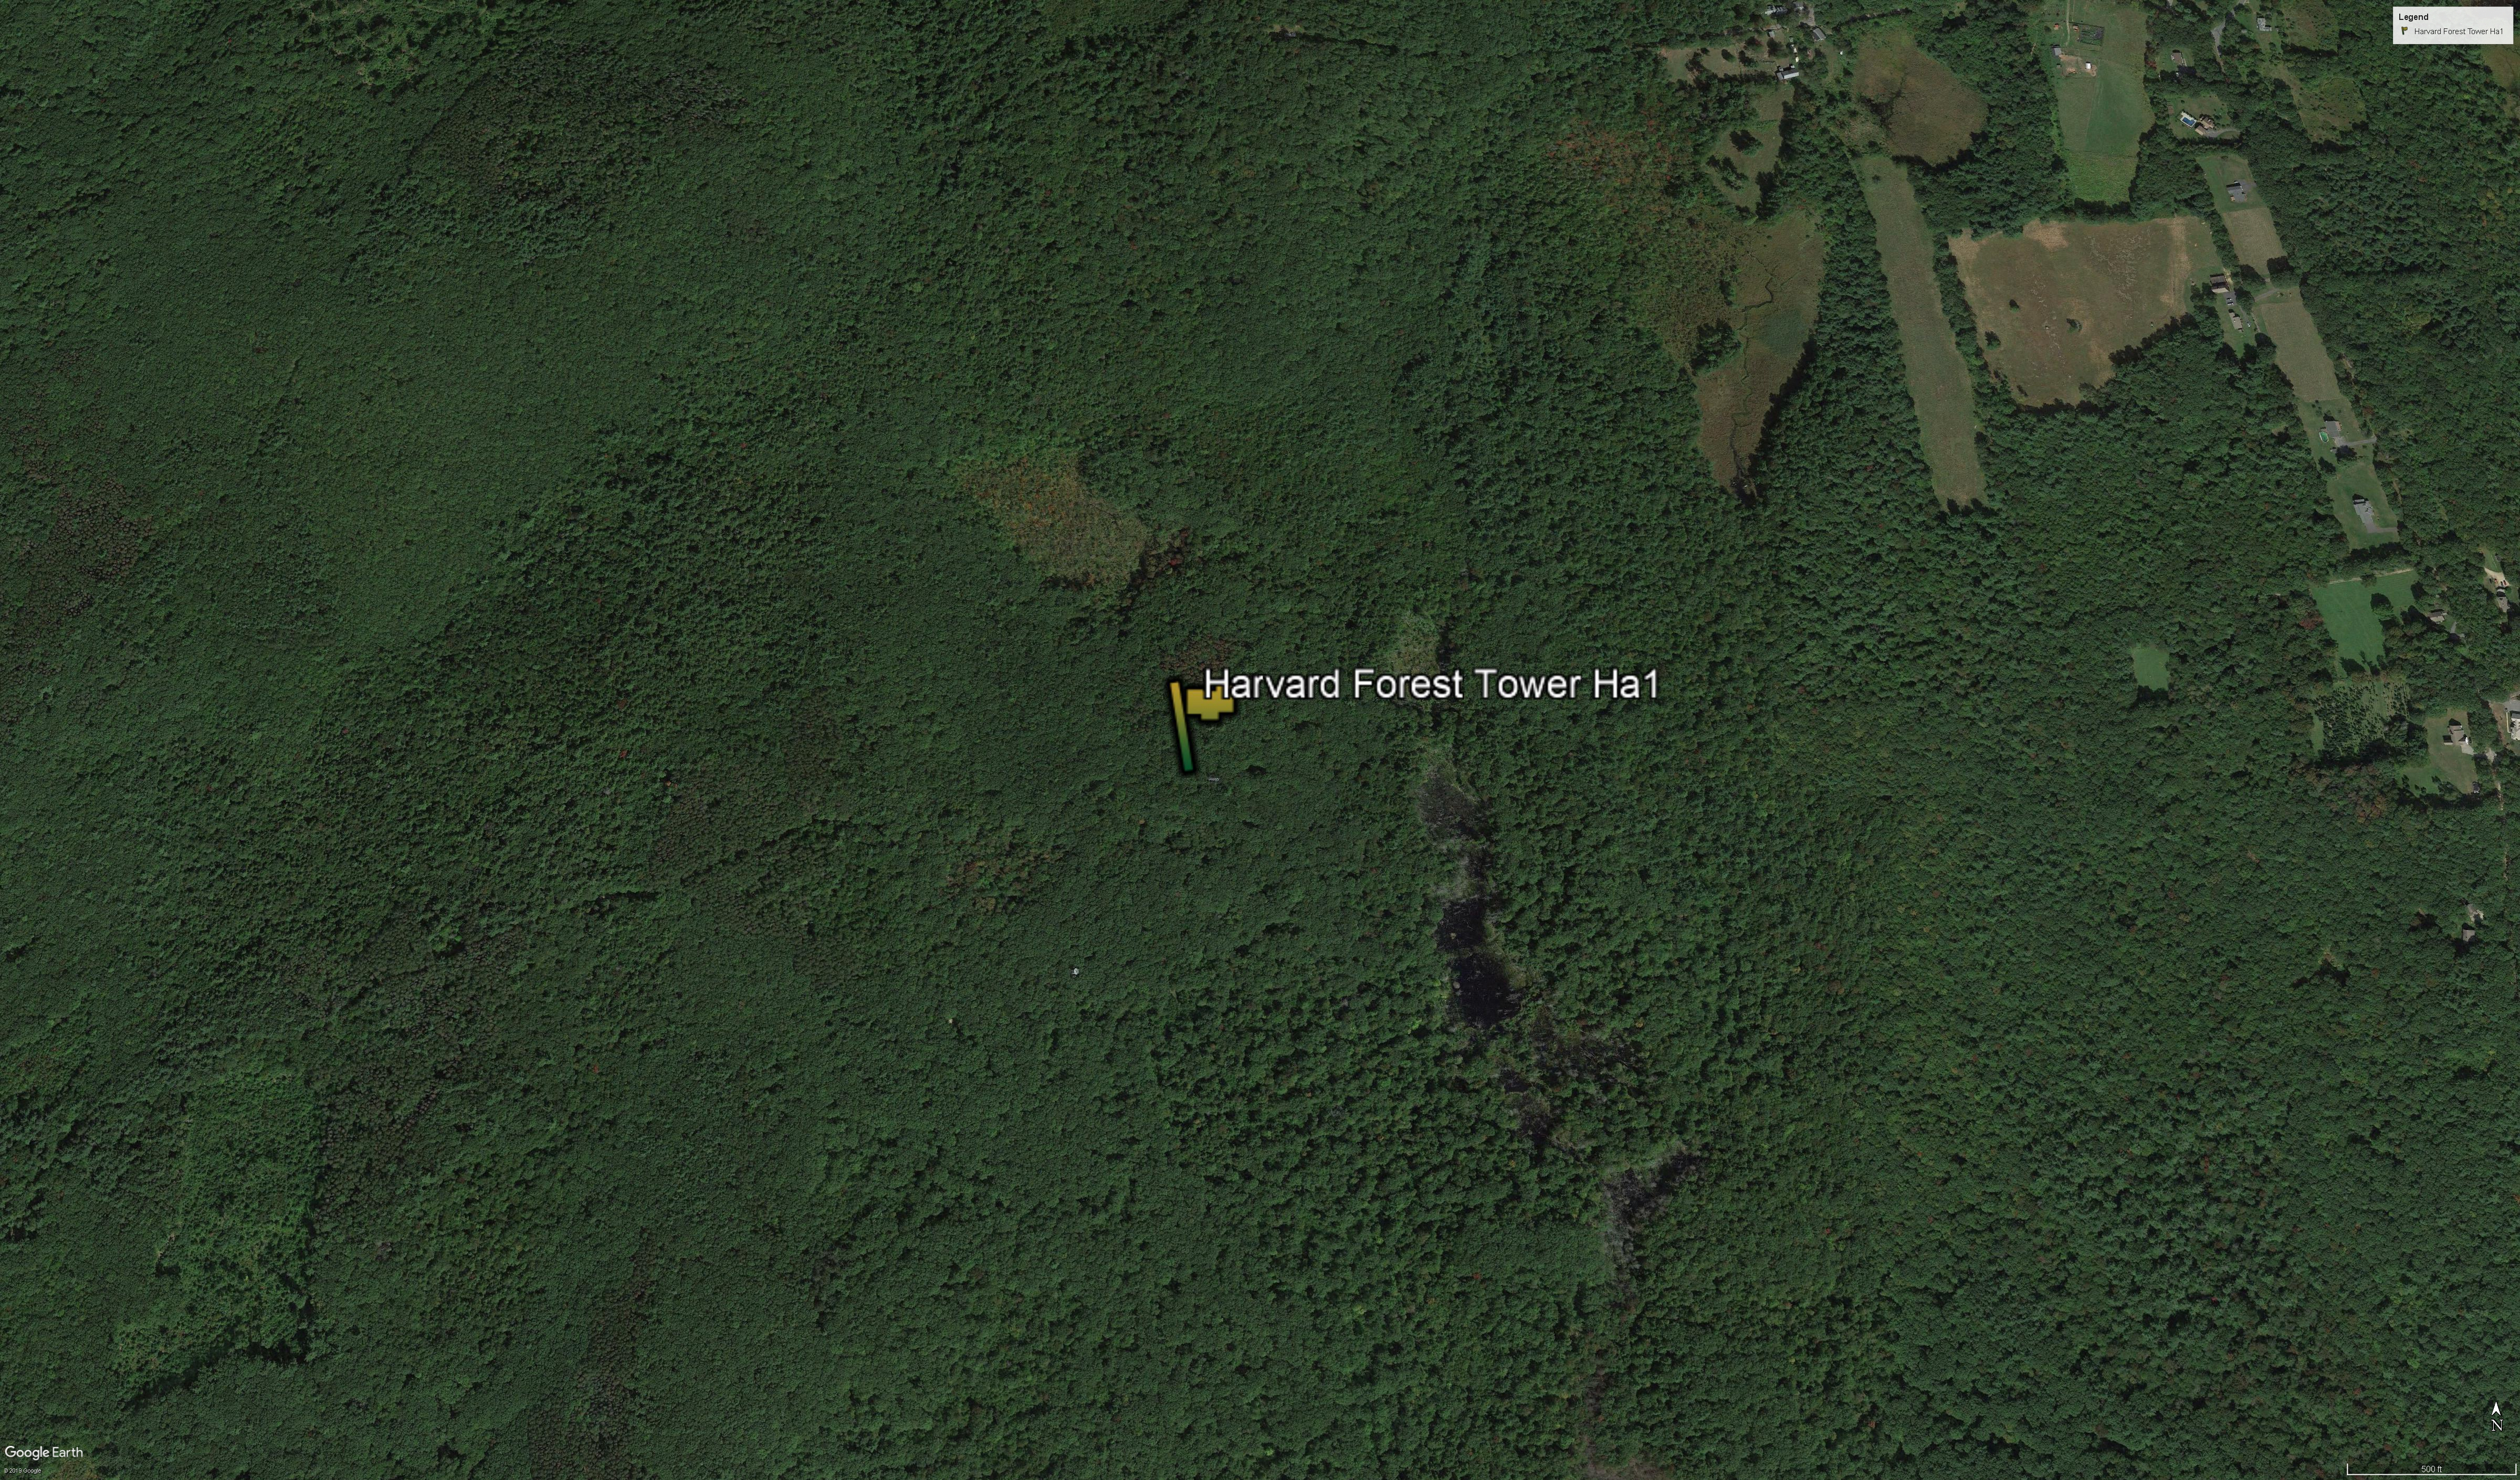
\includegraphics{/Users/katca/Desktop/Reproducible_Science/Image_Harvard.jpg}
\caption{an image caption Source: Harvard Forest tower Ha1 among
temperate forest.}
\end{figure}

A nonlinear least-square (nls) estimator was used for the estimation of
the parameters observed for harv night dataframe, and parms.Month. A
function was created to observe temperature, this was done to measure
variables a, the base respiration when air temperature is 0 degrees
Celsius, and b, an empirical coefficient. Starting values were
identified for the nonlinear model by using selfStart. A function was
created to fit the mofel for temperature: trcModel \textless-
function(TA, a, b) \{ y=a * exp(b*TA) return(y) \}

Then, a function was created to calculate initla values from the data.
Maximum and minimum NEE were found for variables a and b. These
procedures were completed to move on to utilizing the selfStart
function.

The selfStart function created was: SS.trc \textless-
selfStart(model=trcModel,initial= trc.int)

Initial values (iv) for respiration and empirical coefficient were found
for harv harv night dataframe for the month of December.

Assumptions checked were: Residuals vesus fitted values, standardized
residuals, autocorrelation, and histogram (normality).

Bootstrapping was then utilized to estimate errors, and data was
plotted.

\#Results (at least 1 plot and one table)

\#Discussion (1 paragrapgh)

\end{document}
